%intro.tex
\ifx\allfiles\undefined
\documentclass[UTF8, onecolumn, a4paper]{article}

\begin{document}
\fi
\lstset{%代码块全局设置
	backgroundcolor=\color{red!3!green!3!blue!3},%代码块背景色为浅灰色
	rulesepcolor= \color{gray}, %代码块边框颜色
	breaklines=true,  %代码过长则换行
	numbers=left, %行号在左侧显示
	numberstyle= \small,%行号字体
	%keywordstyle= \color{red},%关键字颜色
	commentstyle=\color{gray}, %注释颜色
	frame=shadowbox,%用方框框住代码块
	xleftmargin=1em,
	xrightmargin=0em,
	tabsize=5,
	%rulesepcolor=\color{red!20!green!20!blue!20},  %阴影颜色
	keywordstyle={\color{blue!90!}\fontspec{Consolas Bold}},   %关键字颜色
	commentstyle={\color{blue!70!black}\fontspec{Consolas Italic}},   %注释颜色
	stringstyle=\color{orange!100!black}, %字符串颜色
	numberstyle=\color{purple}, %行号颜色
	%basicstyle=\ttfamily, %代码风格
	basicstyle=\fontspec{Consolas},
	showstringspaces=false,          % underline spaces within strings only  
	showtabs=false,
	captionpos=t, %文件标题位置
	flexiblecolumns
}
\section{Environment and Requirements}
\begin{lstlisting}[title=Environment and Requirements,language=c++]
Intel(R) Core(TM) i7-8750H CPU @ 2.20GHz
Visual Studio 2012, C++: -std=C++11 -O3 -openmp  //算法部分
python==3.7.0  //数据清洗与运行脚本
|- networkx==2.4
|- python_louvain.egg==info
|- matplotlib==3.1.2
|- numpy==1.18.2
|- demjson==2.2.4
|- tqdm==4.45.0
|- requests==2.23.0 //for tranlation
|- community==1.0.0b1
bootstrap@3.3.7 + jQuery@3.4.1 + d3.v3.js  //前端
\end{lstlisting}
\section{Usage}
\begin{lstlisting}[title=Usage]
usage: main.py [-h] [--n N] [--t] [--s]
optional arguments:
-h, --help  show this help message and exit
--n N       number of nodes to build graph
--t         enable translation (en->ch), this needs network connection and
			may take much time
--s         show quantitative information of statistical graph
\end{lstlisting}
\section{File Structure}
\tikzstyle{every node}=[draw=black,thick,anchor=west]
\tikzstyle{selected}=[draw=red,fill=red!30]
\tikzstyle{optional}=[dashed,fill=gray!50]
\begin{center}
	\begin{tikzpicture}
	[grow via three points={one child at (0.5,-0.7) and
		two children at (0.5,-0.7) and (0.5,-1.4)},
	edge from parent path={(\tikzparentnode.south)  |-(\tikzchildnode.west)}]
	\node {刘泓尊\_刘禹潇\_图分析大作业}
	child { node {data}
		child {node {豆瓣电影}
			child{node {movies.csv}}	
		}
		child [missing] {}	
		child {node {论文}
			child{node {papers.csv}}
		}
		child [missing] {}
	}
	child [missing] {}
	child [missing] {}
	child [missing] {}
	child [missing] {}
	child { node {src/Graph/Graph}
		child{node {*.cpp}}
		child{node {*.h}}
	}
	child [missing] {}				
	child { node {static}
		child {node {css/*.css}}
		child {node {img/background.jpg}}
		child {node {js}
			child {node {jquery-3.4.1.min.js}}	
			child {node {movie}
				child {node {info\_nodes.js}}
				child {node {edges.js}}
				child {node {paths.js}}
				child {node {visual\_nodes.js}}
			}
			child [missing] {}				
			child [missing] {}
			child [missing] {}	
			child [missing] {}
			child {node {paper}
				child {node {info\_nodes.js}}
				child {node {edges.js}}
				child {node {paths.js}}
				child {node {visual\_nodes.js}}
			}
		}
	}
	child [missing] {}				
	child [missing] {}
	child [missing] {}				
	child [missing] {}
	child [missing] {}				
	child [missing] {}
	child [missing] {}				
	child [missing] {}
	child [missing] {}	
	child [missing] {}								
	child { node {\textbf{index.html}}}
	child { node {movies.html}}
	child { node {paper.html}}
	child { node {Graph.exe}}
	child { node {main.py}}
	child { node {\textbf{report.pdf}}};
	\end{tikzpicture}
\end{center}
\paragraph{说明:}
图论算法使用C++实现,在VS2012上可以正常运行,放在src/Graph/Graph文件夹下,实现了“最小生成树”,“最短路径”,“两种中心度计算”和提高算法“社群发现”,进行了高度的封装,最终编译成Graph.exe可以从控制台输入数据运行。main.py是完整的运行脚本,包括了\textbf{(a)数据预处理、(b)调用Graph.exe、(c)输出到.js文件}的流程,如果您需要从头开始运行程序,请保持上述文件结构,之后运行main.py即可。观察可视化结果可以打开home.html,网页上提供了转向movies.html和paper.html的链接。


\section{功能展示与说明}
打开home.html文件,该网页介绍了基本的建模方法和跳转链接。点击相应的链接进入可视化界面,您可以点击对应的功能进行测试。
\begin{figure}[htb]
	\centering
	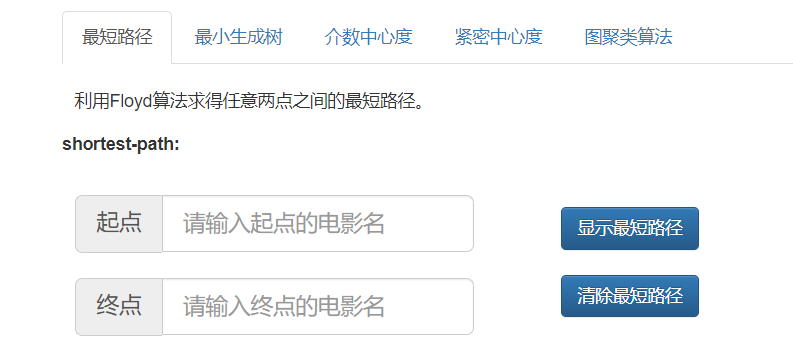
\includegraphics[width=0.6\linewidth]{../pictures/floyd}
	\caption{功能选择栏}
\end{figure}
\paragraph*{}
   下面我们将分别展示“最小生成树”,“最短路径”,“两种中心度计算”和提高算法:“社群发现”的可视化效果。从下页图中可以看到图聚类算法可以较为准确的划分社群,“团”的特征十分明显;其他基础功能的实现也比较准确和直观。在网页侧栏展示了论文和电影的基本信息,其中论文标题还提供了指向源网址的链接。更多细节请打开网页home.html查看。
\begin{center}
	\begin{figure}[ht] %强制单栏排版
		\centering %居中
		\begin{minipage}[b]{\linewidth} %整体划分一个0.93倍页面宽度的页面
			\begin{minipage}[b]{0.6\linewidth} %继续划分子页面 每个宽度0.17倍总宽度
				\centering
				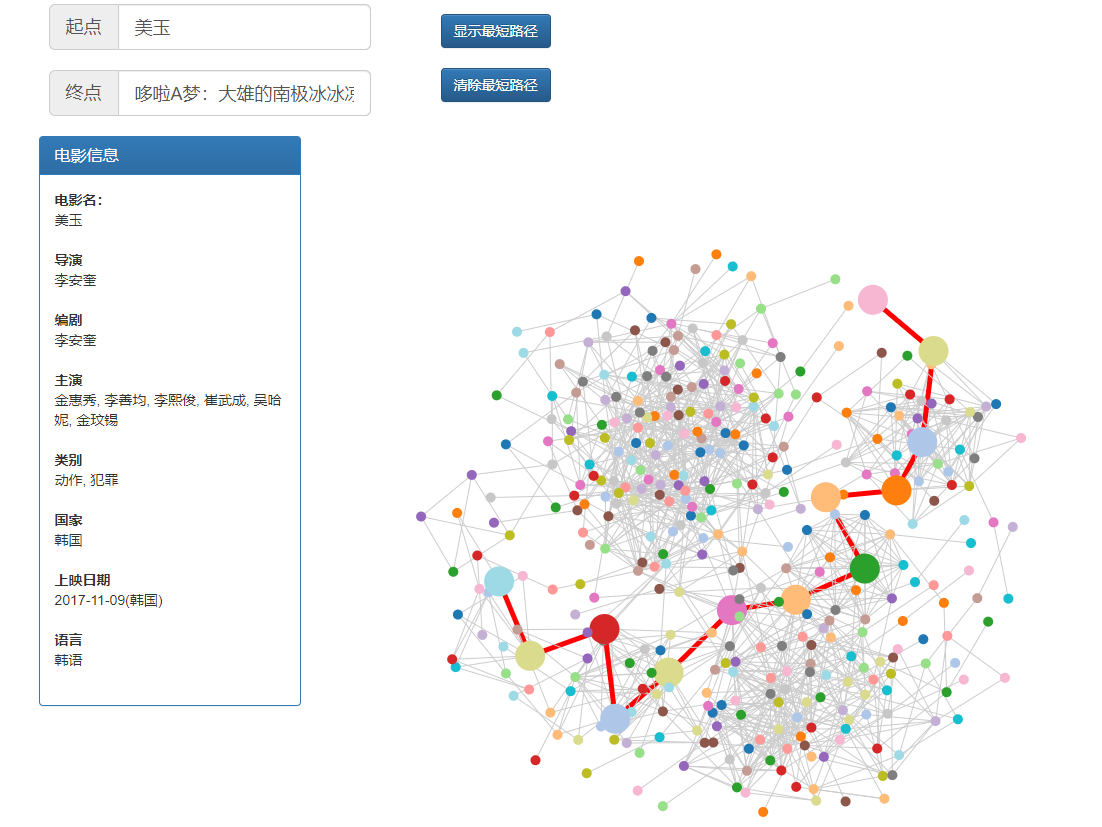
\includegraphics[width=\linewidth]{../pictures/show1}
				\caption{在输入框内输入起点和终点,可以高亮显示最短路径}
			\end{minipage}
			\hfill
			\begin{minipage}[b]{0.4\linewidth}
				\centering
				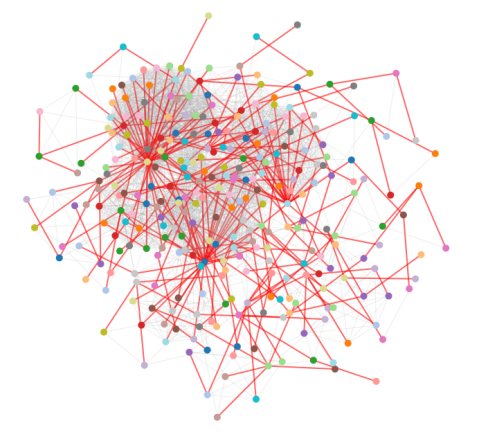
\includegraphics[width=\linewidth]{../pictures/show18}
				\caption{展示最小生成树}
			\end{minipage}
		\end{minipage}
	\end{figure}
\end{center}
\begin{center}
	\begin{figure}[ht] %强制单栏排版
		\centering %居中
		\begin{minipage}[b]{0.93\linewidth} %整体划分一个0.93倍页面宽度的页面
			\begin{minipage}[b]{0.46\linewidth} %继续划分子页面 每个宽度0.17倍总宽度
				\centering
				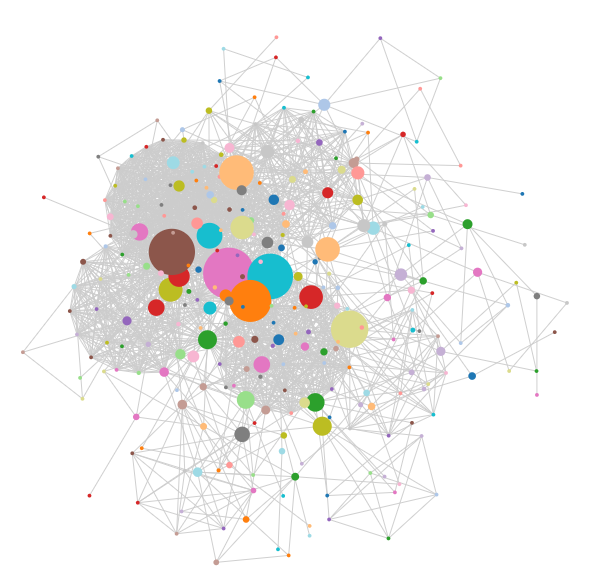
\includegraphics[width=\linewidth]{../pictures/show3}
				\caption{介数中心度展示}
			\end{minipage}
			\hfill
			\begin{minipage}[b]{0.46\linewidth}
				\centering
				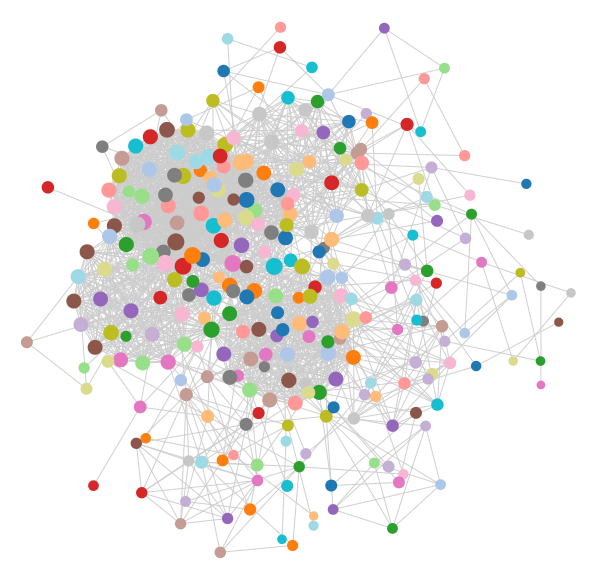
\includegraphics[width=\linewidth]{../pictures/show4}
				\caption{紧密中心度展示}
			\end{minipage}
		\end{minipage}
	\end{figure}
\end{center}
\begin{figure}[htb]
	\centering
	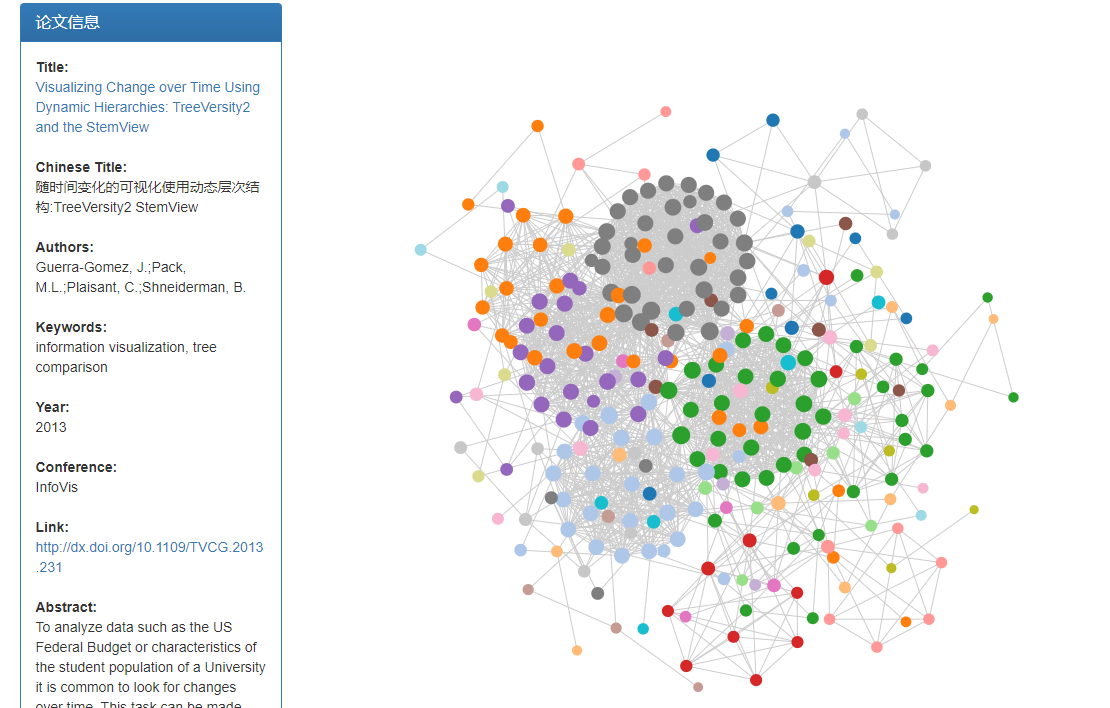
\includegraphics[width=0.8\linewidth]{../pictures/show5}
	\caption{展示图聚类算法}
\end{figure}
\clearpage

\ifx\allfiles\undefined
\end{document}
\fi